%%%%%%%%%%%%%%%%%%%%%%%%%%%%%%%%%%%%%%%%%%%%%%%%%%
\begin{frame}[fragile]{Legacy -- Vermächtnis}
\begin{minipage}{.8 \paperwidth}
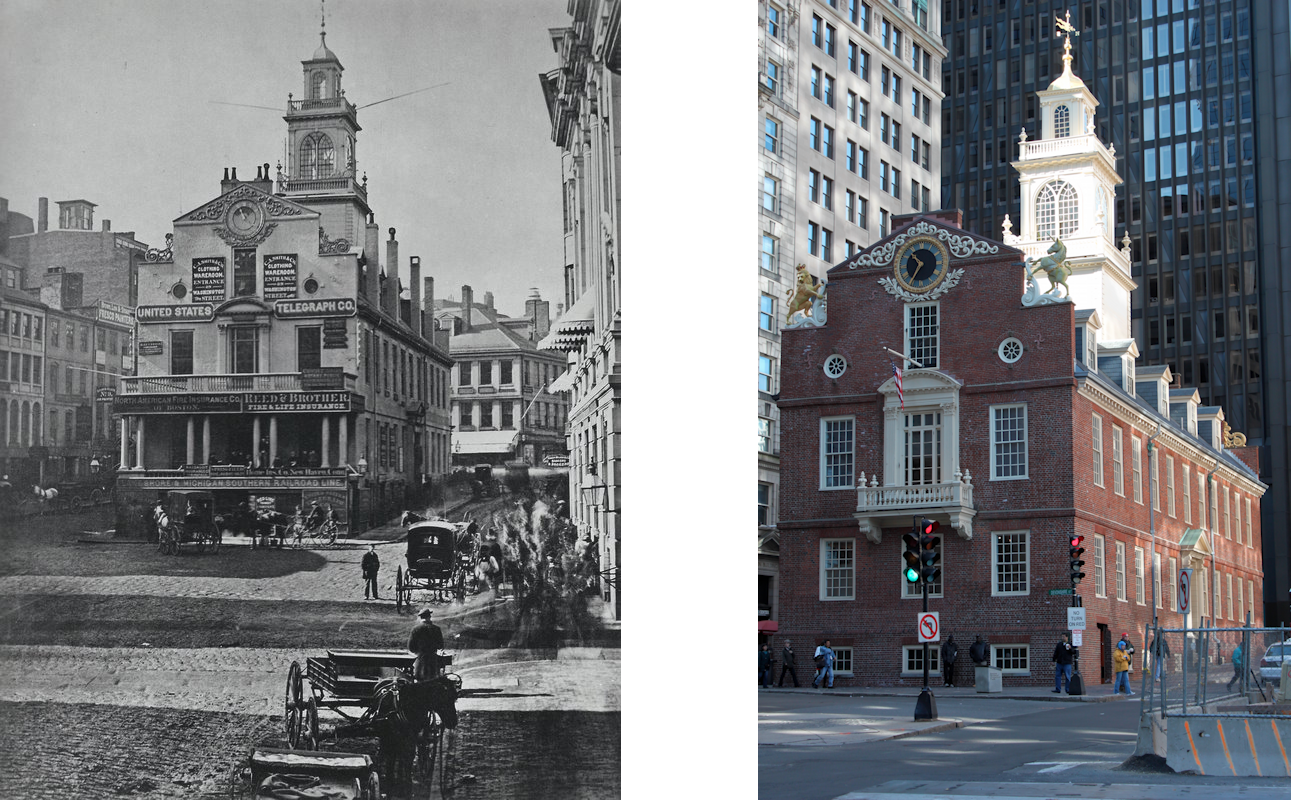
\includegraphics[width=\textwidth]{OldStateHouse.png} \newline
{\tiny \url{http://www.flickr.com/photos/bostonlandmarkscommission/} \hfill \url{http://www.flickr.com/photos/josepha/}}
\end{minipage}
\end{frame}

%%%%%%%%%%%%%%%%%%%%%%%%%%%%%%%%%%%%%%%%%%%%%%%%%%
\begin{frame}[fragile]{Legacy -- Vermächtnis}
\begin{minipage}{.8 \paperwidth}
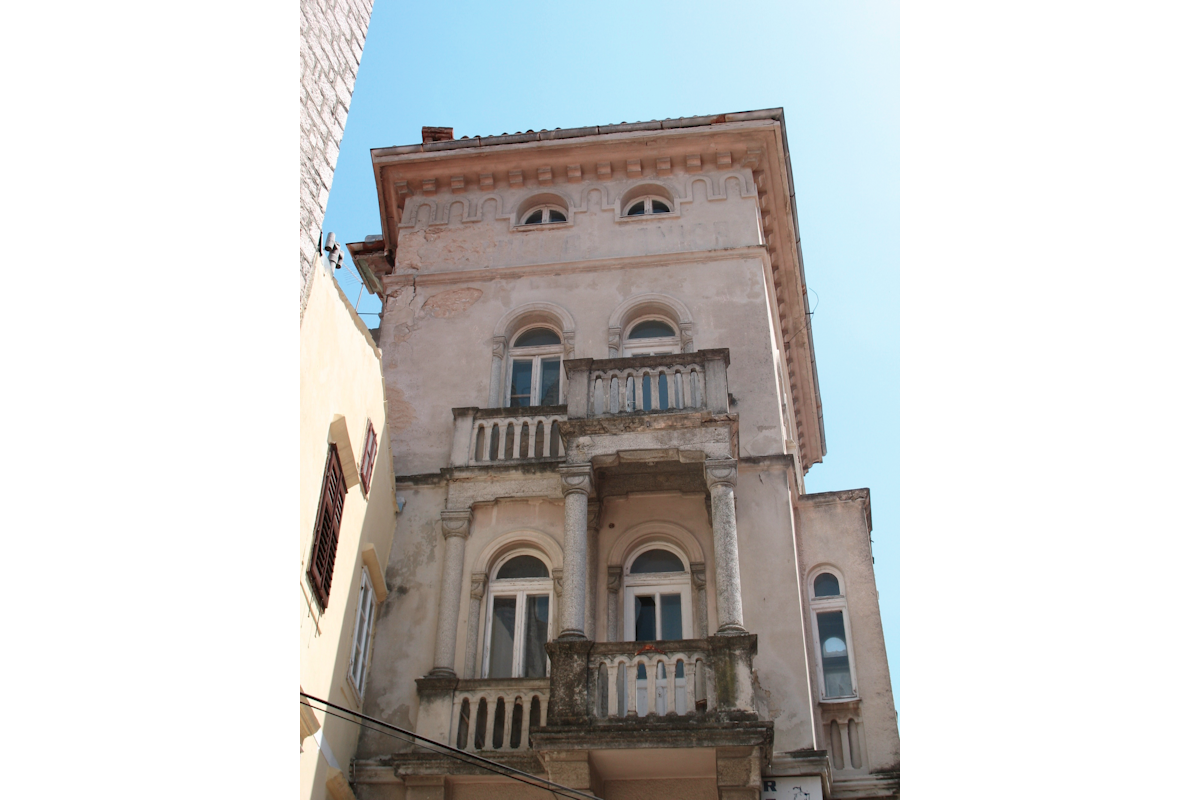
\includegraphics[width=\textwidth]{AlteVilla.png} \newline
{\tiny \hspace*{\fill} \url{http://www.flickr.com/photos/venana/}}
\end{minipage}
\end{frame}

%%%%%%%%%%%%%%%%%%%%%%%%%%%%%%%%%%%%%%%%%%%%%%%%%%
\begin{frame}[fragile]{Legacy -- Vermächtnis}
\begin{minipage}{.8 \paperwidth}
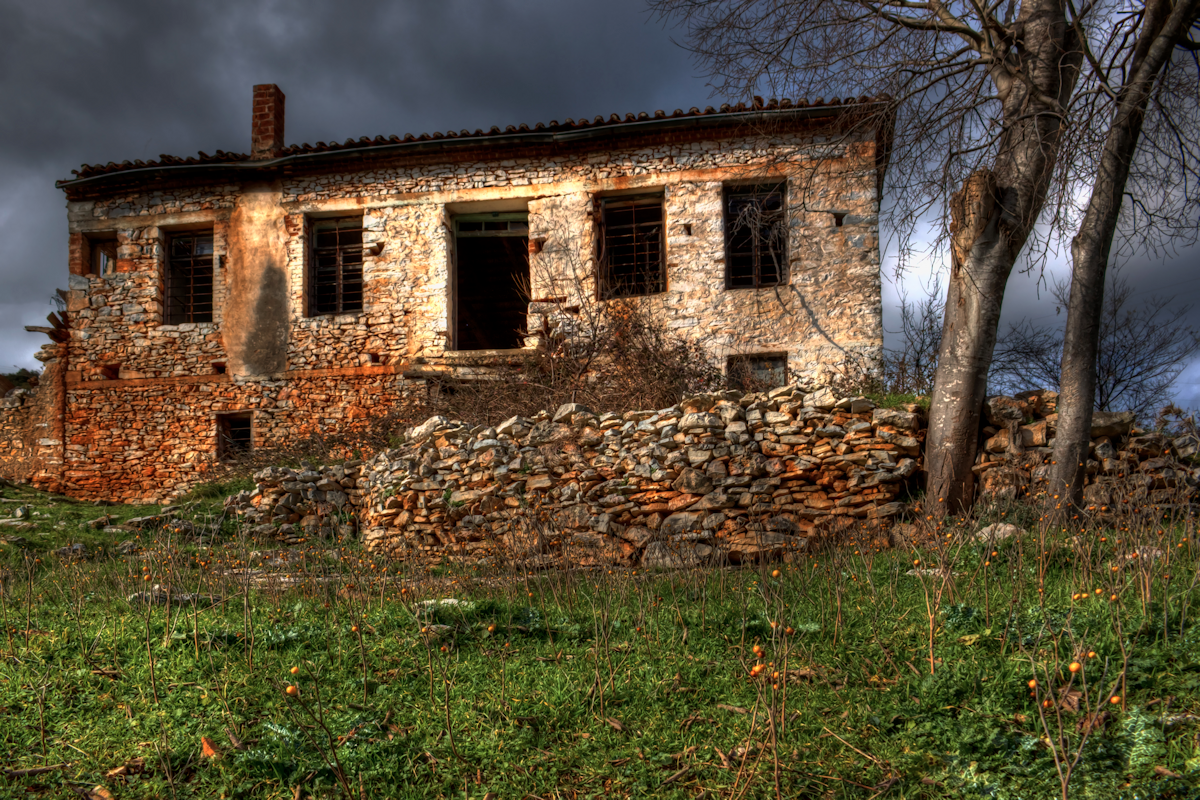
\includegraphics[width=\textwidth]{VerfallenesHaus.png} \newline
{\tiny \hspace*{\fill} \url{http://www.flickr.com/photos/theo_reth/}}
\end{minipage}
\end{frame}

%%%%%%%%%%%%%%%%%%%%%%%%%%%%%%%%%%%%%%%%%%%%%%%%%%
\begin{frame}[fragile]{Legacy Code -- Was ist das eigentlich?}
\begin{itemize}
\item Michael Feathers: \glqq Code without tests\grqq
\begin{itemize}
\item \glqq With tests, we can change the behavior of our code quickly and verifiably.\grqq
\item \glqq Without them, we really don't know if our code is getting better or worse.\grqq
\end{itemize}

\end{itemize}

\end{frame}


%%%%%%%%%%%%%%%%%%%%%%%%%%%%%%%%%%%%%%%%%%%%%%%%%%
\begin{frame}[fragile]{Legacy Code -- Was ist das eigentlich?}
\begin{itemize}
\item Legacy Code ist
\begin{itemize}
\item von anderen
\item alt
\item unübersichtlich
\item buggy
\item mühsam zu erweitern
\item …
\end{itemize}
\end{itemize}

\end{frame}


%%%%%%%%%%%%%%%%%%%%%%%%%%%%%%%%%%%%%%%%%%%%%%%%%%
\begin{frame}[fragile]{Unser Ausgangspunkt}
\begin{itemize}
\item Betriebswirtschaftliche Software
\item Extrem schlechte Codequalität
\item Anstehende Veränderungen für ein Modul:
\begin{itemize}
\item Bugfixing
\item neue Features
\item bessere Tests
\end{itemize}
\end{itemize}

$\Rightarrow$ Ein Umbau war notwendig
\end{frame}

%%%%%%%%%%%%%%%%%%%%%%%%%%%%%%%%%%%%%%%%%%%%%%%%%%
\begin{frame}[fragile]{Vorhandene Codestruktur}
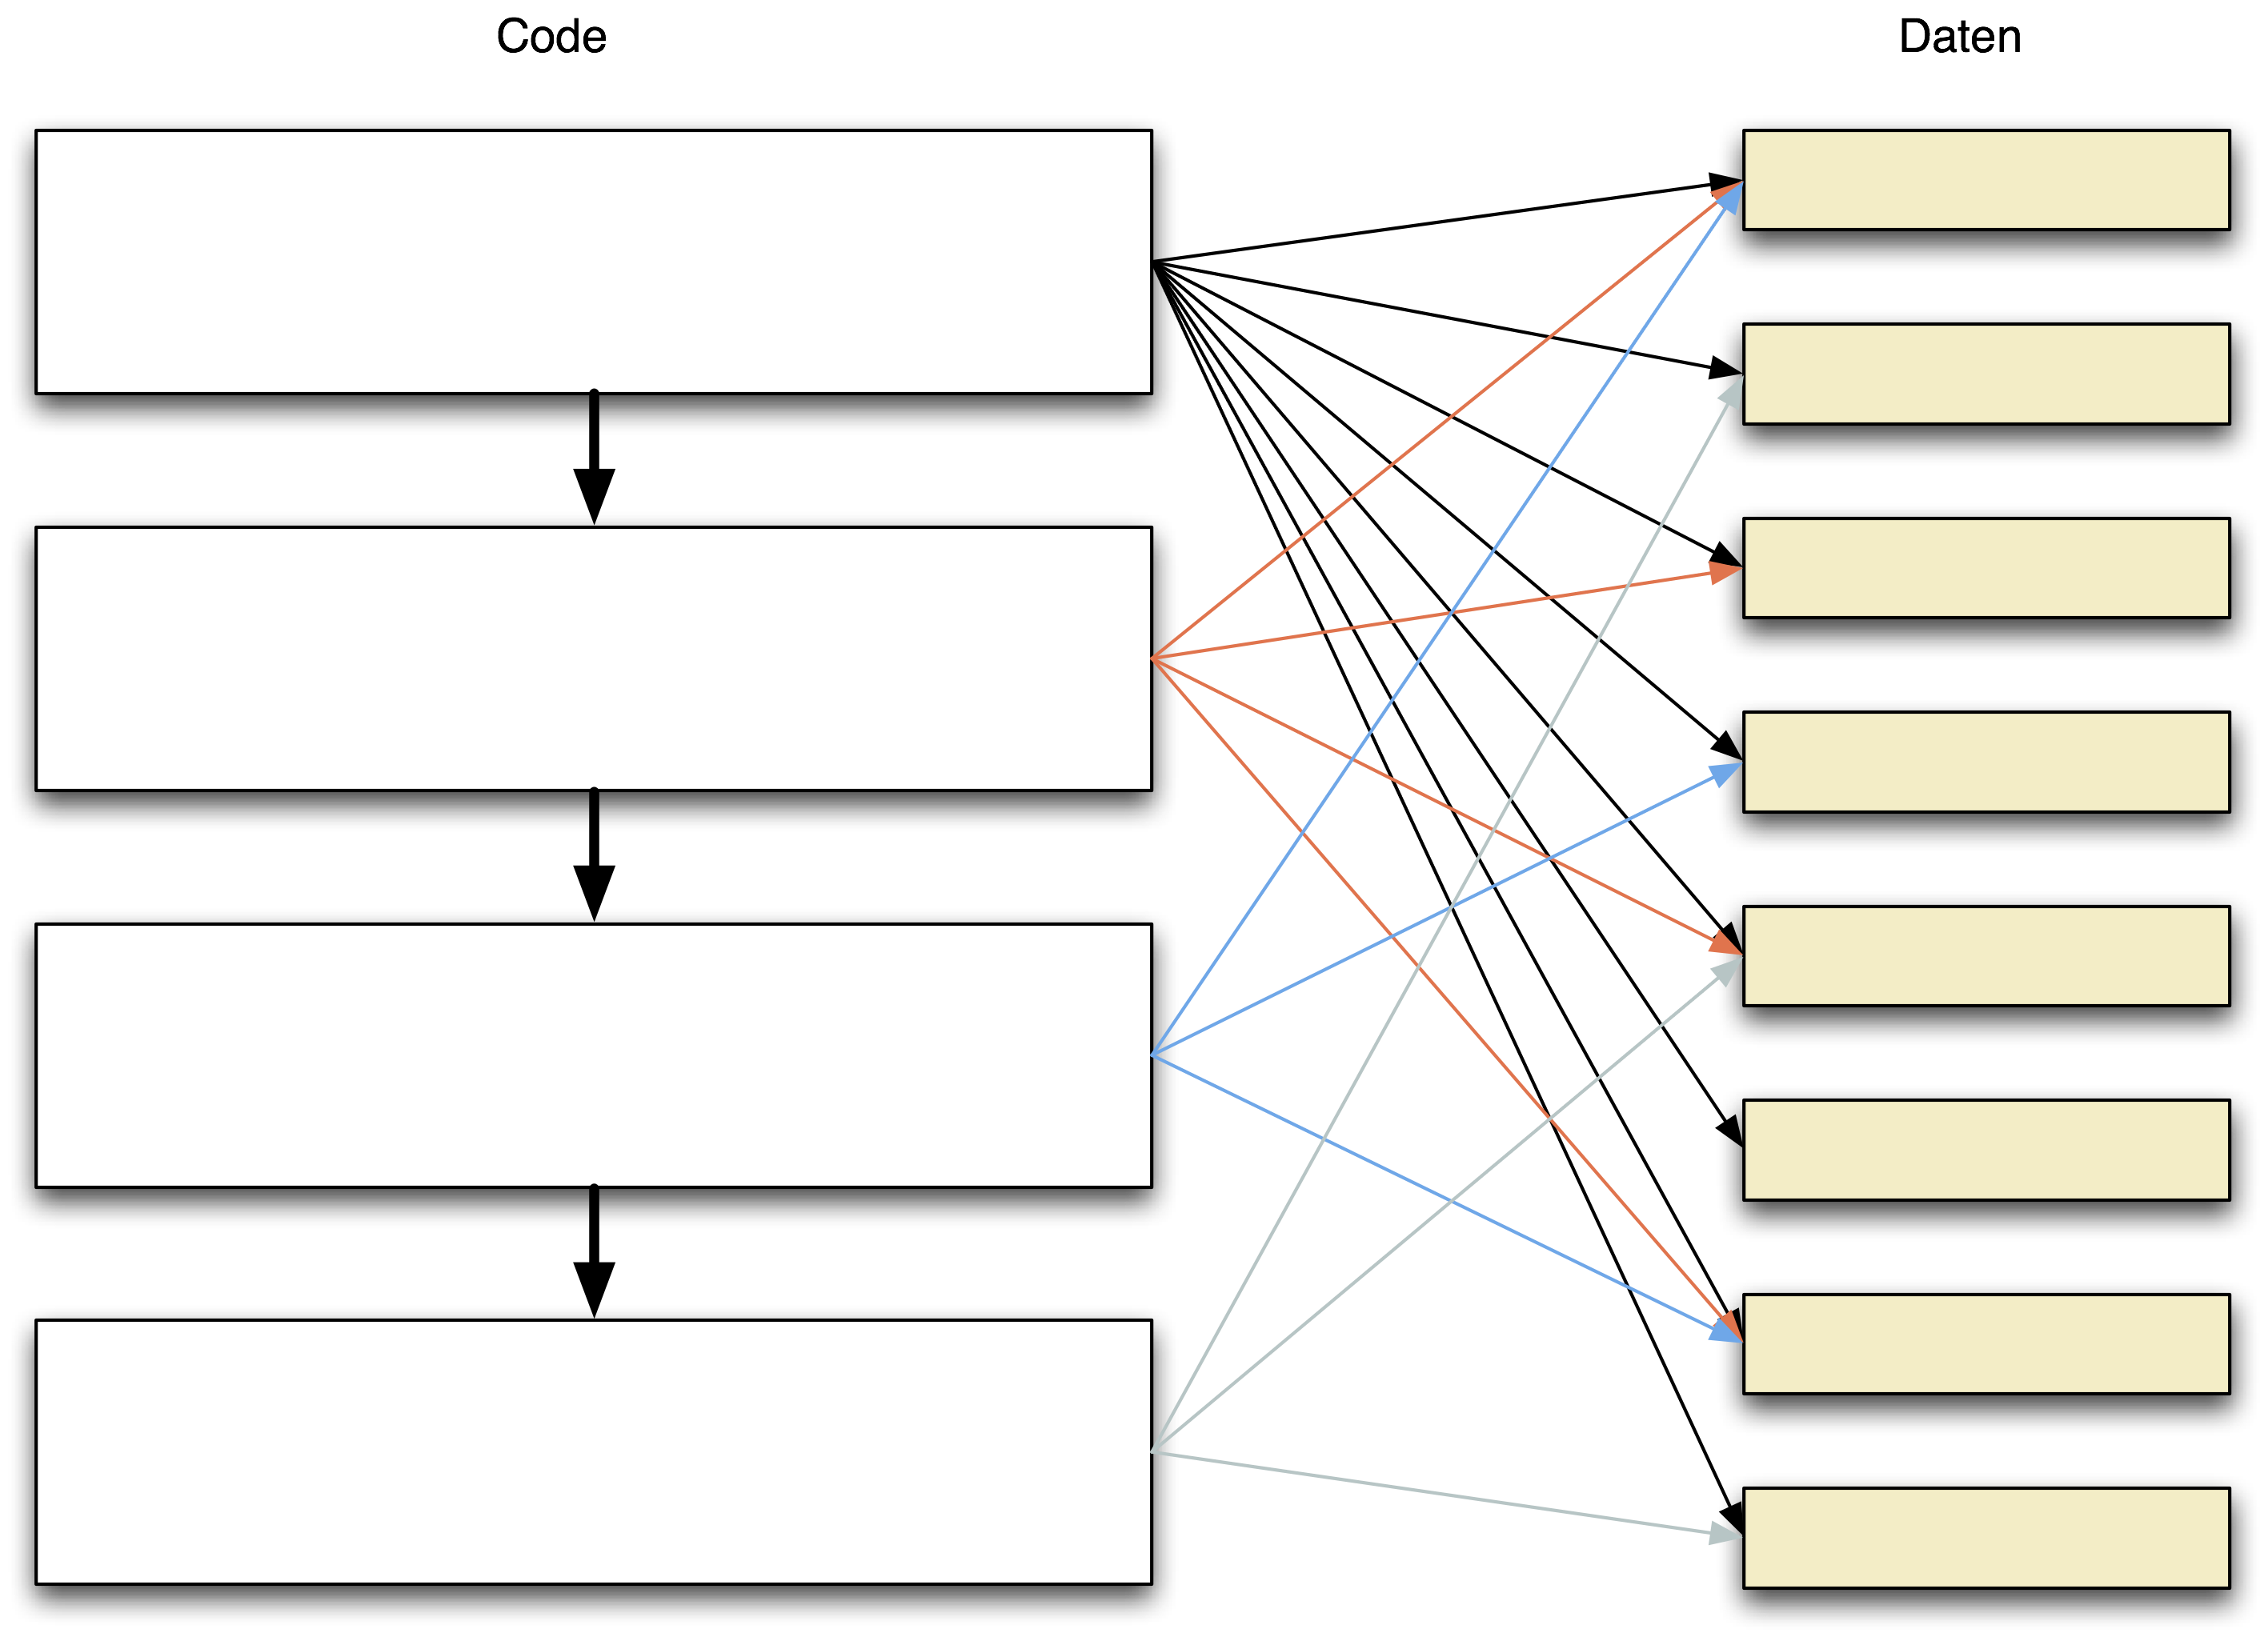
\includegraphics[width=.8 \paperwidth]{Codestruktur.png}
\end{frame}

%%%%%%%%%%%%%%%%%%%%%%%%%%%%%%%%%%%%%%%%%%%%%%%%%%
\begin{frame}[fragile]{Probleme der vorhandenen Codestruktur}
\begin{itemize}
\item Code schreibt Werte in separate Datenobjekte (\glqq Push\grqq{})
\item Mehrfache Schreibzugriffe auf denselben Wert
\item Codeteile greifen auf vorher geschriebene Werte zu
\item Code ist getrieben vom Blick von innen: Was muss ich alles in Summe tun, um eine Menge von Ergebnissen abliefern zu können?
\end{itemize}
\end{frame}



%%%%%%%%%%%%%%%%%%%%%%%%%%%%%%%%%%%%%%%%%%%%%%%%%%
\begin{frame}[fragile]{Unser Ansatz}
\begin{itemize}
\item Annahmen:
\begin{itemize}
\item Der alte Code ist großteils inkorrekt und lückenhaft
\item Es existiert umfassendes Wissen über die gewünschte Fachlogik
\end{itemize}
\end{itemize}

\begin{itemize}
\item Entschluss:
\begin{itemize}
\item Neuimplementierung auf der grünen Wiese (mit Feature-Toggle)
\item Erstellung neuer Tests anhand der parallel zu definierenden Fachlichkeit
\item Kontinuierliche Anpassung der vorhandenen Tests
\end{itemize}
\end{itemize}

\end{frame}


%%%%%%%%%%%%%%%%%%%%%%%%%%%%%%%%%%%%%%%%%%%%%%%%%%
\begin{frame}[fragile]{Unsere Erfahrungen}
\begin{itemize}
\item Probleme:
\begin{itemize}
\item Die Ausarbeitung der fachlichen Spezifikation ist viel komplizierter und aufwändiger als gedacht
\item Abweichungen zum alten Code sind schwer zu analysieren
\item Die Testabdeckung ist zu gering \newline $\Rightarrow$ Wir übersehen relevante Fälle 
\end{itemize}
\end{itemize}

\begin{itemize}
\item Ursachen:
\begin{itemize}
\item Falsche Annahmen
\item Vermischung von Umbau und Änderung
\item Arroganz (\glqq Wir wissen es besser als unsere Vorgänger\grqq{})
\end{itemize}
\end{itemize}

$\Rightarrow$ Wir sind den Umbau viel zu naiv angegangen

\end{frame}


%%%%%%%%%%%%%%%%%%%%%%%%%%%%%%%%%%%%%%%%%%%%%%%%%%
\begin{frame}[fragile]{Wie geht es besser?}
\begin{itemize}
\item Vor dem Umbau Fakten sammeln, Annahmen allein genügen nicht
\begin{itemize}
\item Wie hoch ist die Testabdeckung? (Coverage)
\item Welche fachlichen Fälle sind abgedeckt?
\item Existiert eine zum Code passende Spezifikation?
\end{itemize}

\item Grundsätzlich gilt: Im Zweifel hat der vorhandene Code Recht!

\item Keine Änderungen an der Logik während des strukturellen Umbaus!

\item Explizite Abnahme des Umbaus
\begin{itemize}
\item Das Verhalten muss exakt gleich sein (Tests, Bugs, Features)
\end{itemize}

\end{itemize}
\end{frame}



%%%%%%%%%%%%%%%%%%%%%%%%%%%%%%%%%%%%%%%%%%%%%%%%%%
\begin{frame}[fragile]{Wozu das Ganze?}
\begin{itemize}
\item Struktur:
\begin{itemize}
\item Spiegelbild der Fachlichkeit
\end{itemize}
\end{itemize}

\begin{itemize}
\item Blick von außen aus Sicht der Ergebnisse:
\begin{itemize}
\item Welche Werte will ich haben?
\item Wie berechnet sich welcher Wert?
\item Welche Kategorien von Ergebniswerten gibt es? Gemeinsamkeiten, Unterschiede?
\end{itemize}
\end{itemize}
\end{frame}


%%%%%%%%%%%%%%%%%%%%%%%%%%%%%%%%%%%%%%%%%%%%%%%%%%
\begin{frame}[fragile]{Ideale Vorgehensweise}
\begin{itemize}
\item Feature-Toggle zum Vergleichen von alter und neuer Version
\begin{itemize}
\item Identifikation bzw. Schaffen eines minimalen Eingriffspunkts
\item Beibehalten der externen API an diesem Eingriffspunkt
\end{itemize}
\end{itemize}

\begin{itemize}
\item Wichtige Aspekte des Umbaus:
\begin{itemize}
\item Fachlich motiviert
\item Rein strukturell
\end{itemize}
\end{itemize}

\begin{itemize}
\item Technisches Ziel:
\begin{itemize}
\item Separation of Concerns
\item On-Demand-Ermittlung aller Werte (\glqq Pull\grqq{})
\item Werte-Caching mittels Lazy-Initialization
\end{itemize}

\end{itemize}
\end{frame}



%%%%%%%%%%%%%%%%%%%%%%%%%%%%%%%%%%%%%%%%%%%%%%%%%%
\begin{frame}[fragile]{Umbau: Vorbereitung}
\begin{itemize}
\item Existierenden Code duplizieren
\item Feature Toggle an den Aufrufstellen einbauen
\end{itemize}
\end{frame}
 
%%%%%%%%%%%%%%%%%%%%%%%%%%%%%%%%%%%%%%%%%%%%%%%%%%
\begin{frame}[fragile]{Vorarbeiten}
\begin{itemize}
\item Java-Datumsarithmetik kapseln, z.~B.
\begin{itemize}
\item Joda Time
\item Eigene Klassen
\end{itemize}
\end{itemize}

\begin{itemize}
\item Namensgebung von Variablen verbessern
\end{itemize}
\end{frame}

%%%%%%%%%%%%%%%%%%%%%%%%%%%%%%%%%%%%%%%%%%%%%%%%%%
\begin{frame}[fragile]{Strukturellen Code isolieren}
\begin{itemize}
\item Schleifen aufräumen, vereinheitlichen und zusammenfassen
\item Dazu bei Bedarf Methoden inlinen
\end{itemize}
\end{frame}

%%%%%%%%%%%%%%%%%%%%%%%%%%%%%%%%%%%%%%%%%%%%%%%%%%
\begin{frame}[fragile]{Aspekte isolieren}
\begin{itemize}
\item Werteobjekt einführen, das alle relevanten Ergebnisse des Schleifenrumpfs zusammenfasst
\item Schleifenrumpf in Methode extrahieren
\item Methode in das Werteobjekt verschieben
\end{itemize}
\end{frame}

%%%%%%%%%%%%%%%%%%%%%%%%%%%%%%%%%%%%%%%%%%%%%%%%%%
\begin{frame}[fragile]{Push in Pull umwandeln}
\begin{itemize}
\item Pro Ergebniswert ein Duplikat dieser Methode
\item Jeweils Irrelevantes aus den Methoden entfernen
\item Die Methoden zum Berechnen der Ergebniswerte in Getter umwandeln
\item Parallel dazu Unit-Tests aufbauen
\end{itemize}
\end{frame}

%%%%%%%%%%%%%%%%%%%%%%%%%%%%%%%%%%%%%%%%%%%%%%%%%%
\begin{frame}[fragile]{Vervollständigung}

\begin{itemize}
\item Refactoring: 
\begin{itemize}
\item Extrahieren von Methoden
\item Zusammenfassen gleicher Funktionalität
\item Generelle Aufräumarbeiten
\end{itemize}
\end{itemize}

\begin{itemize}
\item Danach: 
\begin{itemize}
\item Technische Bereinigung von Algorithmen, fachliche Korrektur der Berechnungslogik
\end{itemize}
\end{itemize}

\end{frame}

%%%%%%%%%%%%%%%%%%%%%%%%%%%%%%%%%%%%%%%%%%%%%%%%%%
{
\usebackgroundtemplate{
\includegraphics[width=\paperwidth,height=\paperheight]{background-slide.png}}
\begin{frame}{Vielen Dank!}

        Code \& Folien auf GitHub:
        \begin{center}
                \url{https://github.com/NicoleRauch/RefactoringLegacyCode}
        \end{center}

        \begin{block}{Andreas Leidig}
        \begin{description}[Twitterxx]
                \item[E-Mail]  \href{mailto:andreas.leidig@msg-gillardon.de}{\texttt{andreas.leidig@msg-gillardon.de}}
                \item[Twitter] \href{http://twitter.com/leiderleider}{\texttt{@leiderleider}}
        \end{description}
        \end{block}

        \begin{block}{Nicole Rauch}
        \begin{description}[Twitterxx]
                \item[E-Mail]  \href{mailto:nicole.rauch@msg-gillardon.de}{\texttt{nicole.rauch@msg-gillardon.de}}
                \item[Twitter] \href{http://twitter.com/NicoleRauch}{\texttt{@NicoleRauch}}
        \end{description}
        \end{block}
\end{frame}
}
